\chapter{Tarea 2}

% TAREA 2.

%     Visualiza el siguiente vídeo:

% https://www.google.com/search?client=firefox-b-d&q=Kaspersky+Industrial+CyberSecurity+demonstration+for+Energy+sector+-+Bing+video+#fpstate=ive&vld=cid:fc74c561,vid:7LNtjWx17mA,st:0


\framedt{Tarea a realizar}{

   Visualiza el siguiente vídeo:
   \href{
      https://www.youtube.com/watch?v=7LNtjWx17mA
   }{youtube.com/watch?v=7LNtjWx17mA}
   
   \begin{itemize}
   	\item Identifica en la red industrial los componentes físicos, ciberfísicos, y ciber
	\item Identifica los tipos de ataque que se describen en el vídeo, y explica brevemente como piensas que se podrían implementar.
	\item Explica cómo plantea la solución de Kaspersky en el vídeo la defensa frente a los posibles ataques.
   \end{itemize}
}


%     Contesta a las siguientes preguntas:

%     Identifica en la red industrial que se describe en el vídeo:

% a. Lo componentes físicos

% b. Los componentes ciberfísicos

% c. Los componentes ciber

%     Identifica los tipos de ataque que se describen en el vídeo, y explica brevemente como piensas que se podrían implementar.

%     Explica cómo plantea la solución de Kaspersky en el vídeo la defensa frente a los posibles ataques.

\begin{figure}[htbp]
   \centering
   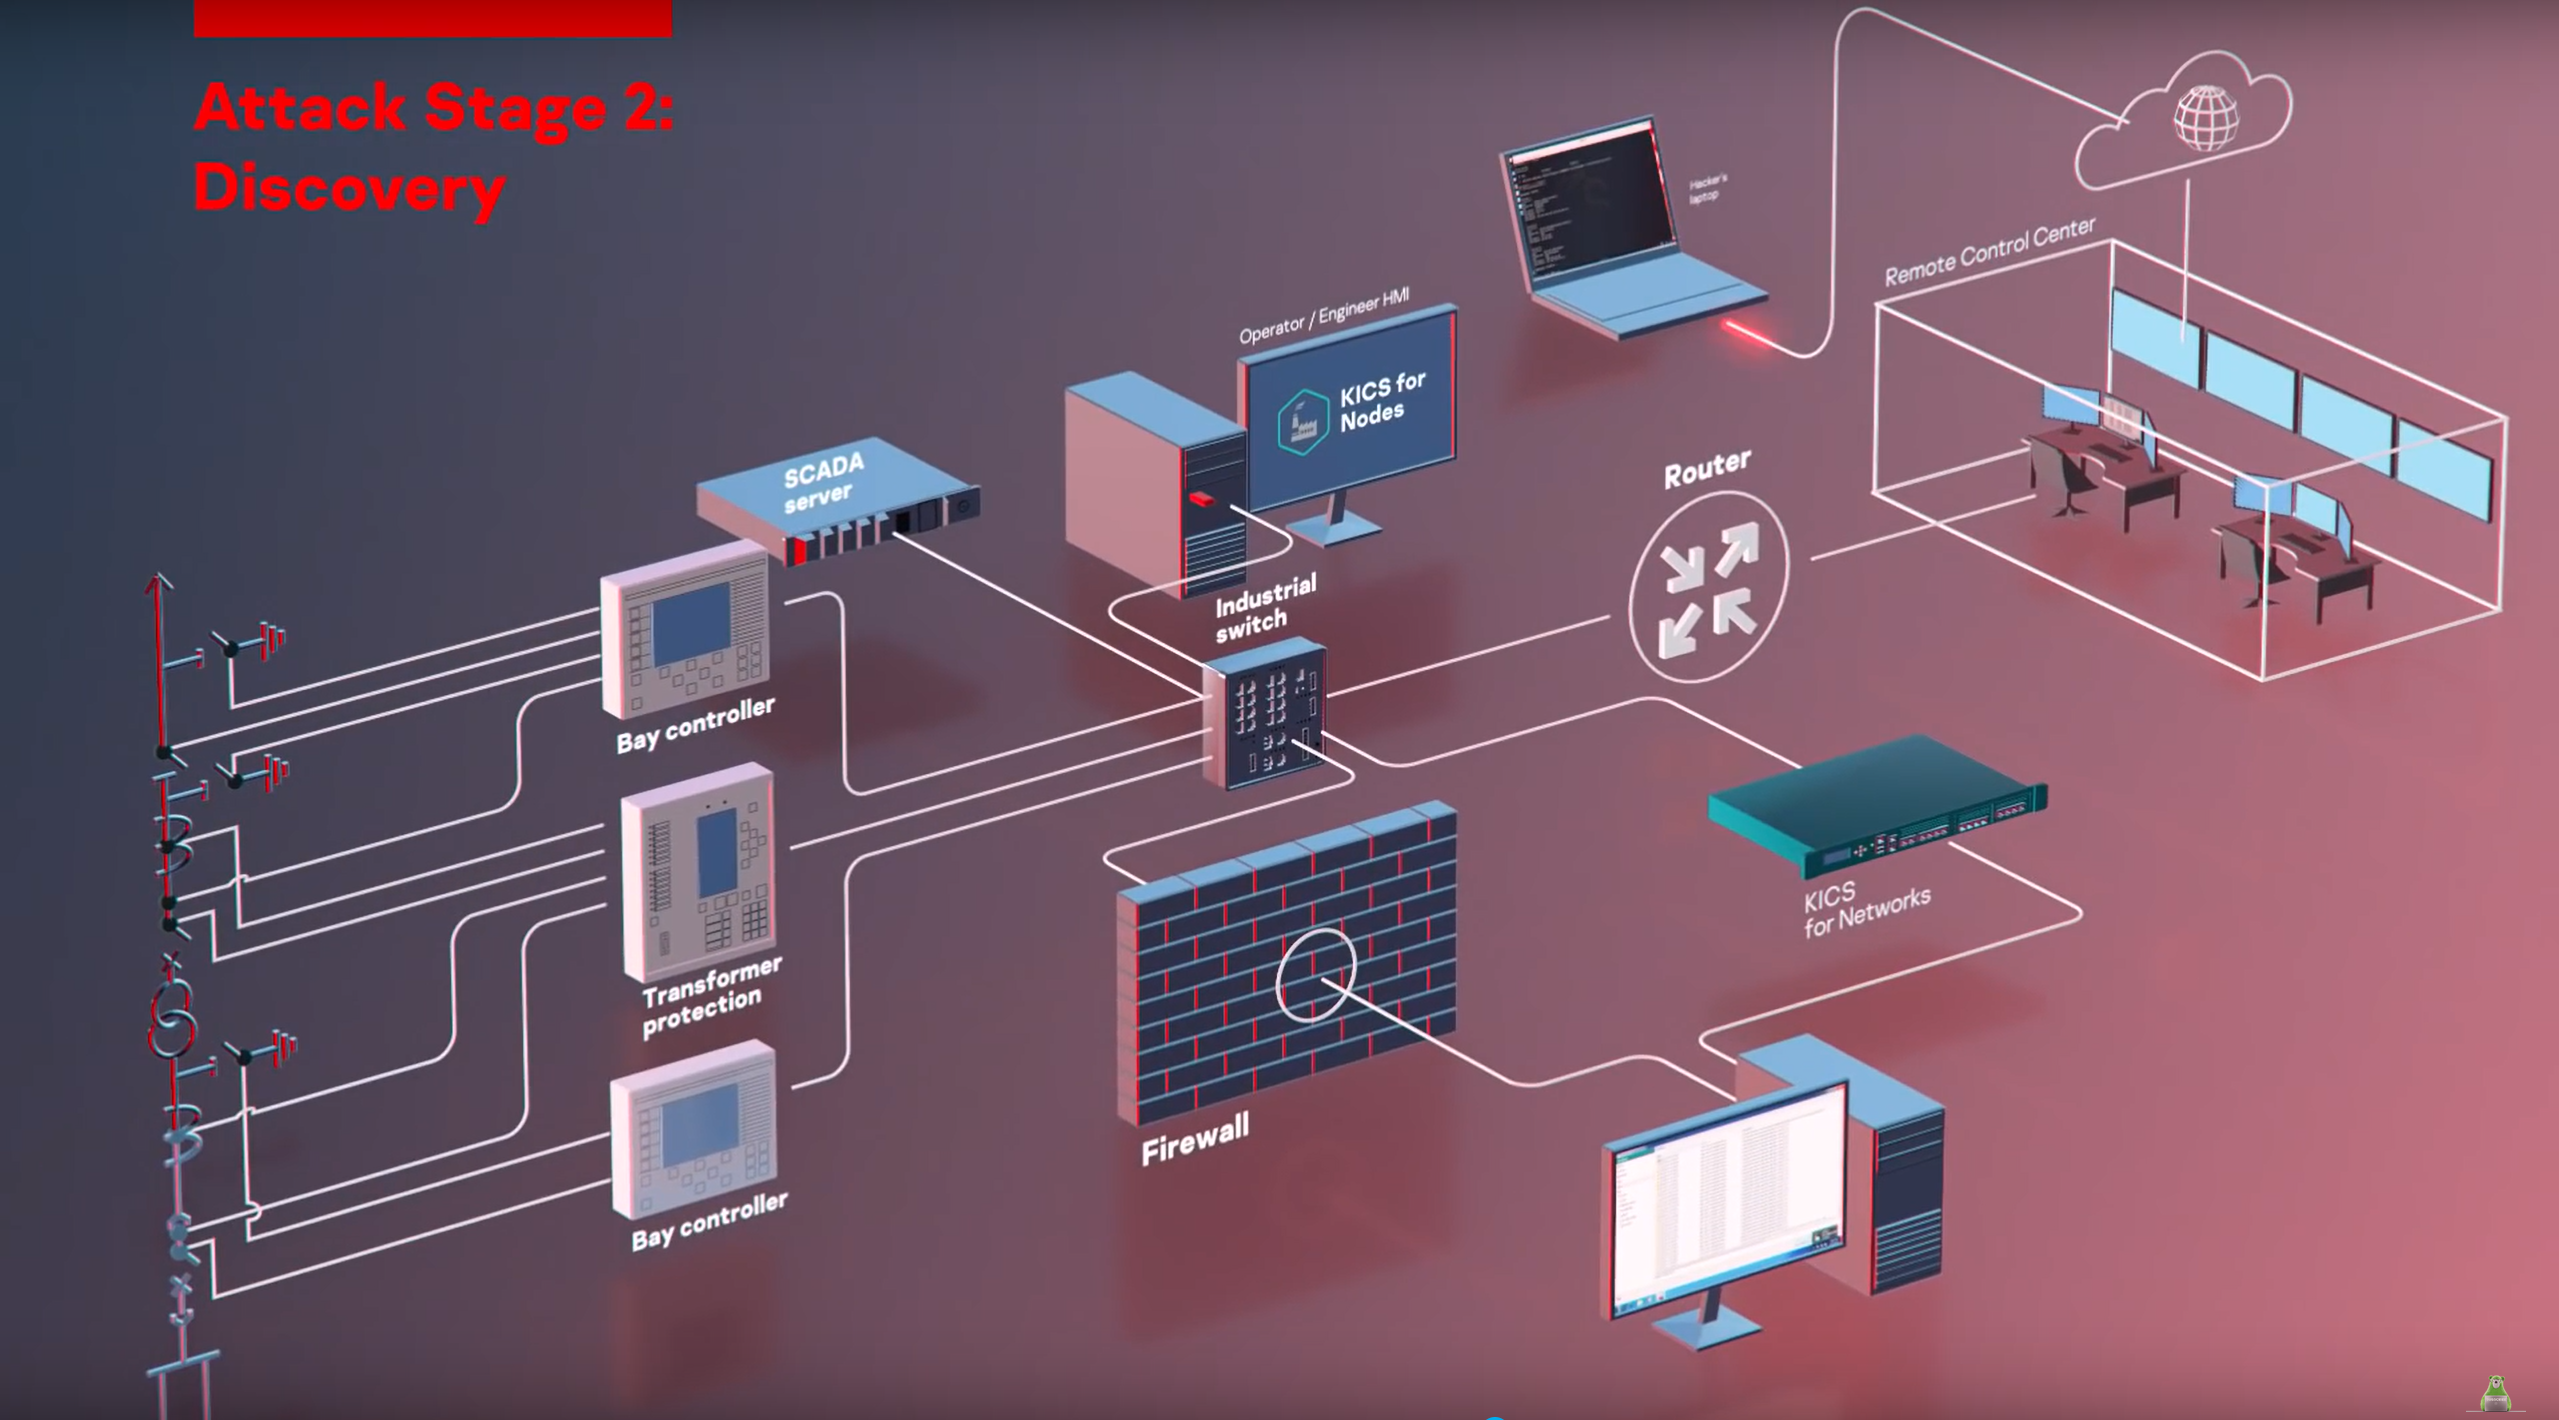
\includegraphics{images/ICSscenario.png}
   \caption{Escenario representado en el vídeo}
   \label{fig:ICSscenario}
\end{figure}


\section{Componentes de la red industrial}

\begin{itemize}
   \item \textbf{Componentes físicos:}
   \begin{itemize}
      \item 100kv high-voltage incoming line
      \item Power transformer
      \item 10kV bus feeder
      \item Primary switching equipment
   \end{itemize}
   \item \textbf{Componentes ciberfísicos:}
   \begin{itemize}
      \item transformer protection
      \item 2 bay controllers
      \item Industrial Ethernet switch
   \end{itemize}
   \item \textbf{Componentes ciber:}
   \begin{itemize}
      \item Kaspersky Industrial CyberSecurity
      \begin{itemize}
         \item \textsc{KICS} for Nodes - Endpoint Protection
         \item \textsc{KICS} for Network - Anomaly and Breach Protection
         \item Centralized security management
         \item Kasperky Security Center - Manager installed on nodes
      \end{itemize}
      \item Router
      \item Firewall
      \item Remote Control Center tools
      \item SCADA server
   \end{itemize}
\end{itemize}

\subsection{Kaspersky Industrial CyberSecurity (\textsc{KICS})}
% Software / hardware / virtual appliance
\begin{paracol}{2}
   
   Las ---``claimed''--- features de \textsc{KICS} son las siguientes:
   \begin{itemize}
	\item Passive traffic analysis
	\item No influence on network stability
	\item Detection of:
	\begin{itemize}
      \item Unauthorized network access
      \item Cyberattacks and intrusions
      \item Unauthorized commands to industrial equipment
      \item Technological parameters anomalies:
      \begin{itemize}
         \item Rules based
	      \item Machine learning
      \end{itemize}
      \item Assets and its parameters
      \item Abnormal dataflow on network map
   \end{itemize}
\end{itemize}

\switchcolumn

\colfill
\begin{figure}[htbp]
   \centering
   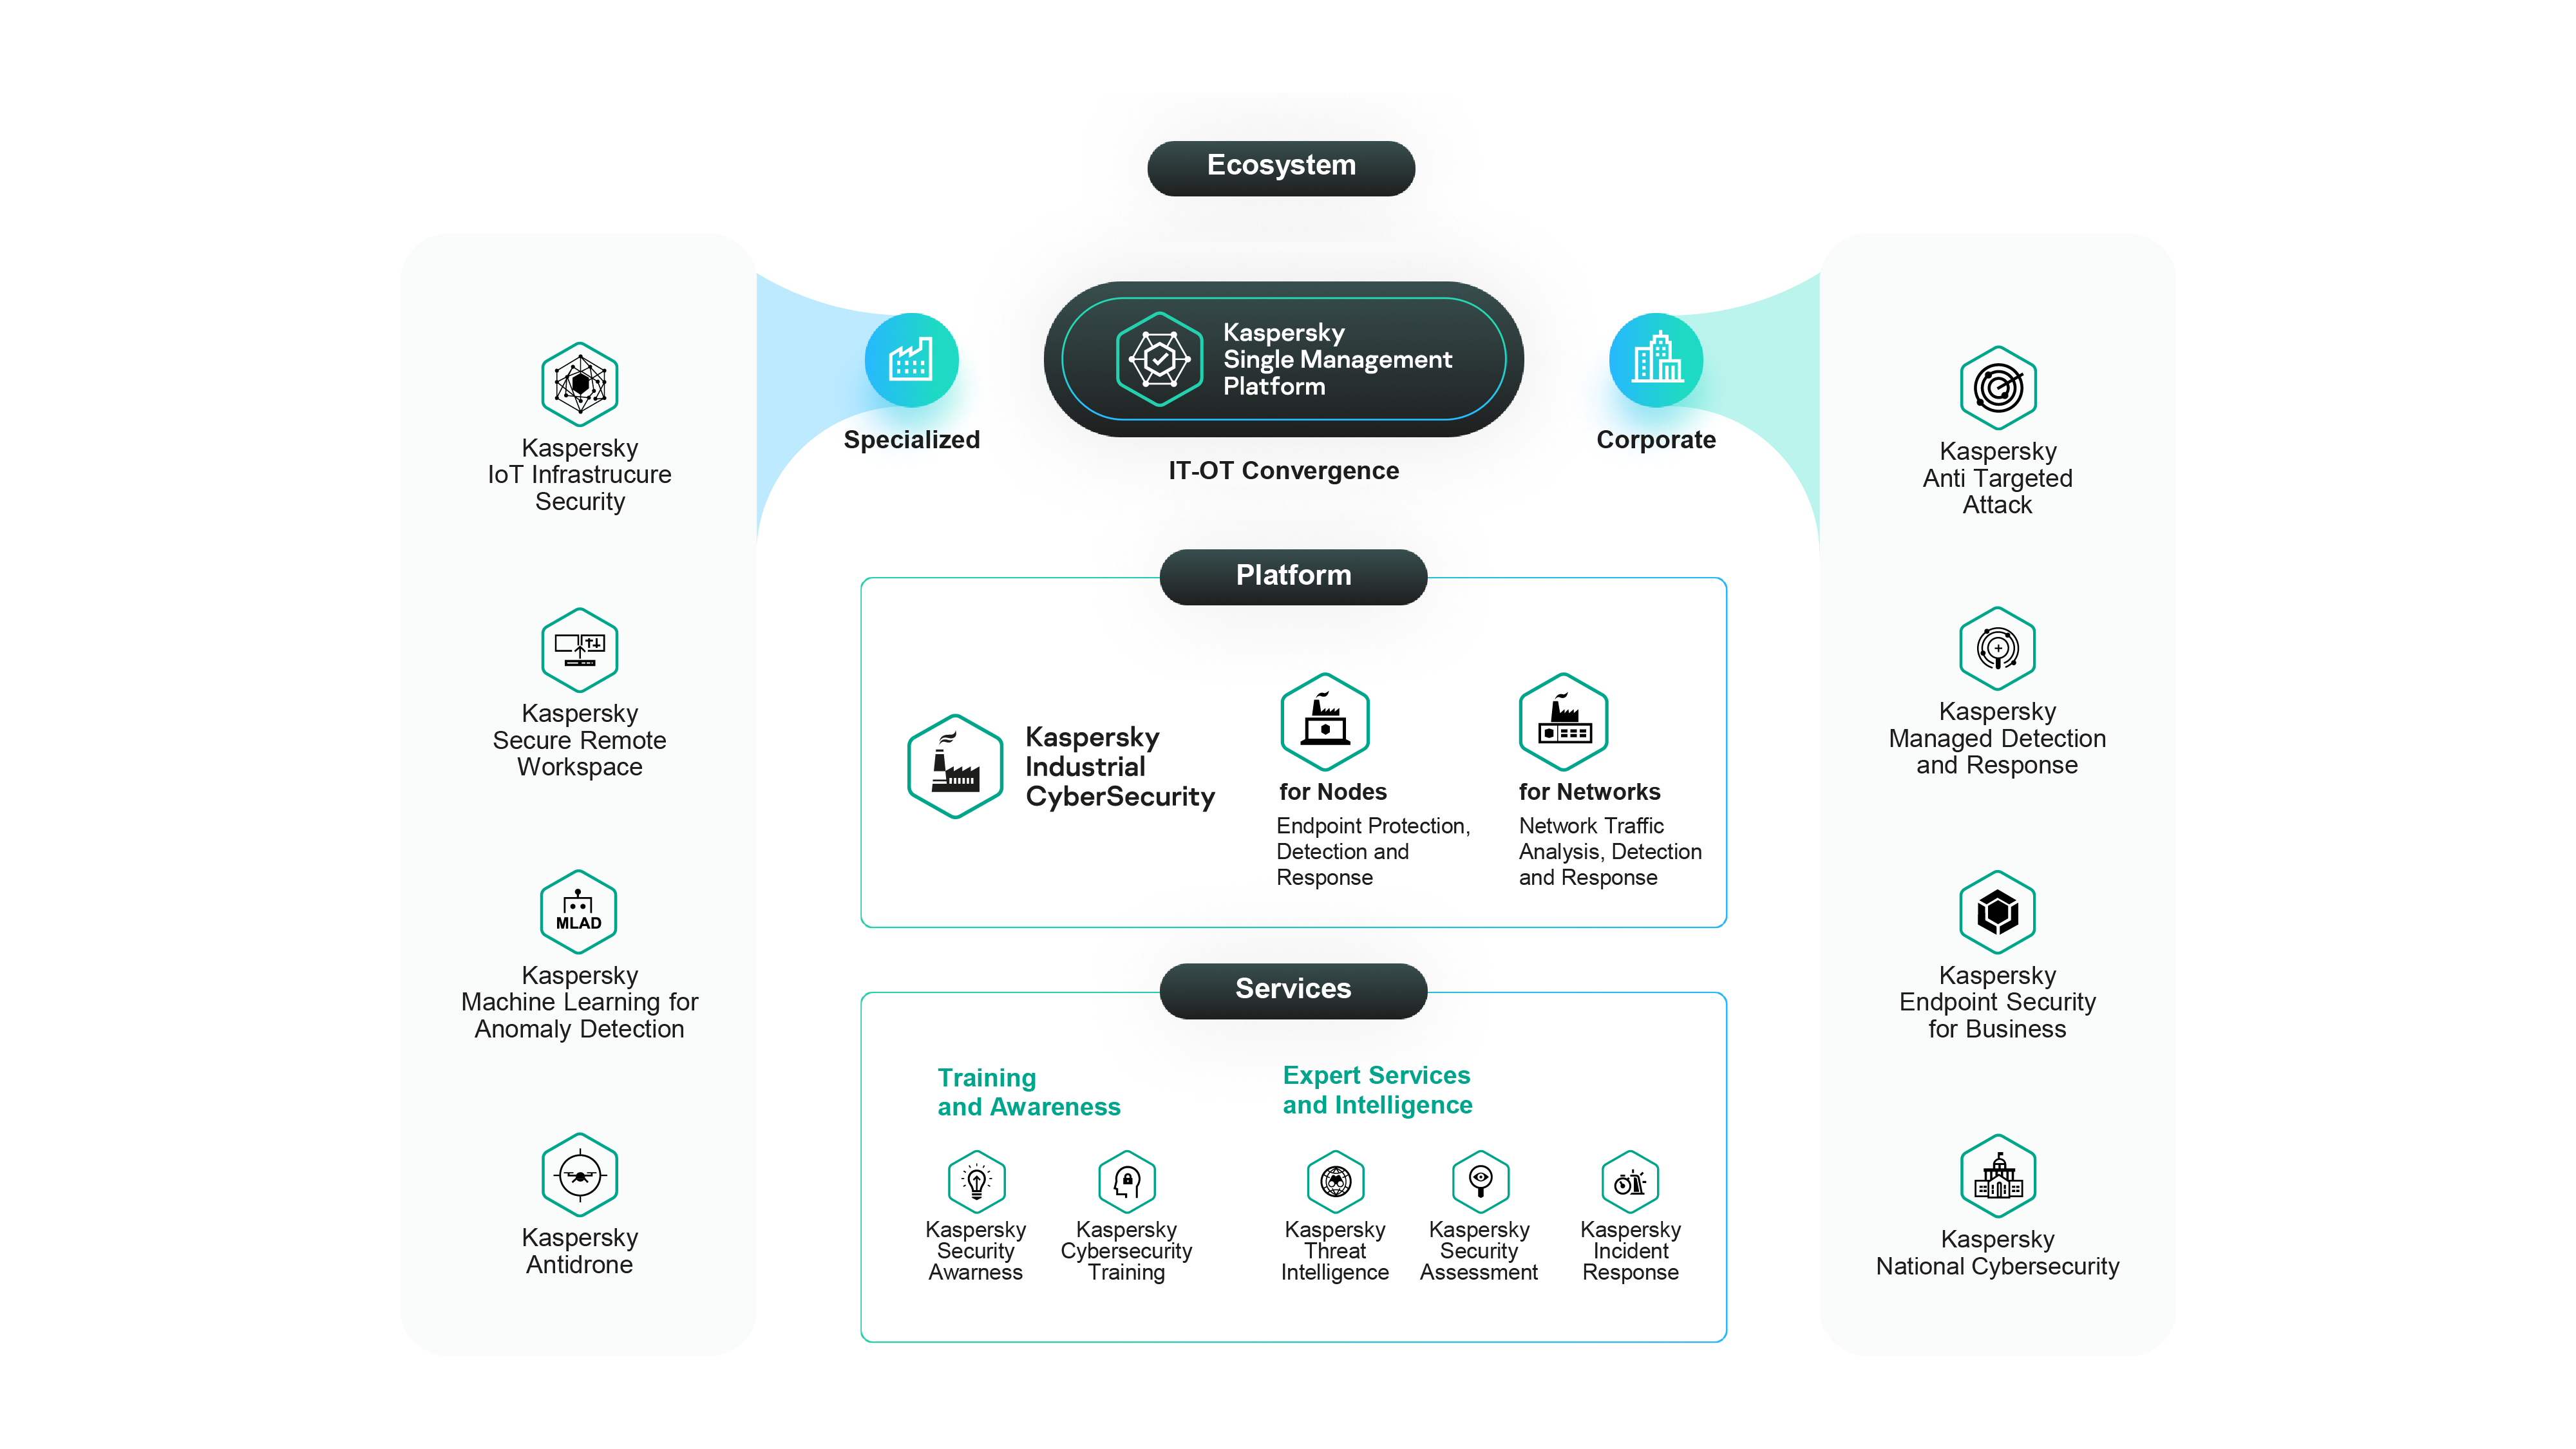
\includegraphics[width=0.95\columnwidth]{images/KICS.png}
   \caption{\textsc{KICS} schema}
   \label{fig:KICS}
\end{figure}
\colfill

\end{paracol}
\section{Ataque sobre la infraestructura industrial y defensa}

El ataque que se muestra en el video comprende tres fases, también se analizan las posibles implementaciones de cada una de ellas:
\begin{enumerate}
   \item \textbf{Breach} - \textit{Obtener acceso a un componente}
   \begin{itemize}
      \item Instalar un malware a traves de un documiento \texttt{.pdf} en un \textsc{usb}, que cuando se abre, se conecta al atacante, que obtiene acceso la computadora infectada, que puede utilizar como fuente para futuros ataques en la red.
      \item \textit{\ul{Defensa}} - \textsc{KICS} for Networks detecta una comunicación no autorizada entre la computadora infectada y una dirección IP externa y un payload potencialmente peligroso, y envía una alerta a \textit{Kaspersky Security Center}.
      \note{Si puede bloquear el ataque aquí, pero en el video se supone que no lo haces para mostrar el comportamiento defensivo en las fases siguientes}
      \begin{figure}[htbp]
         \centering
         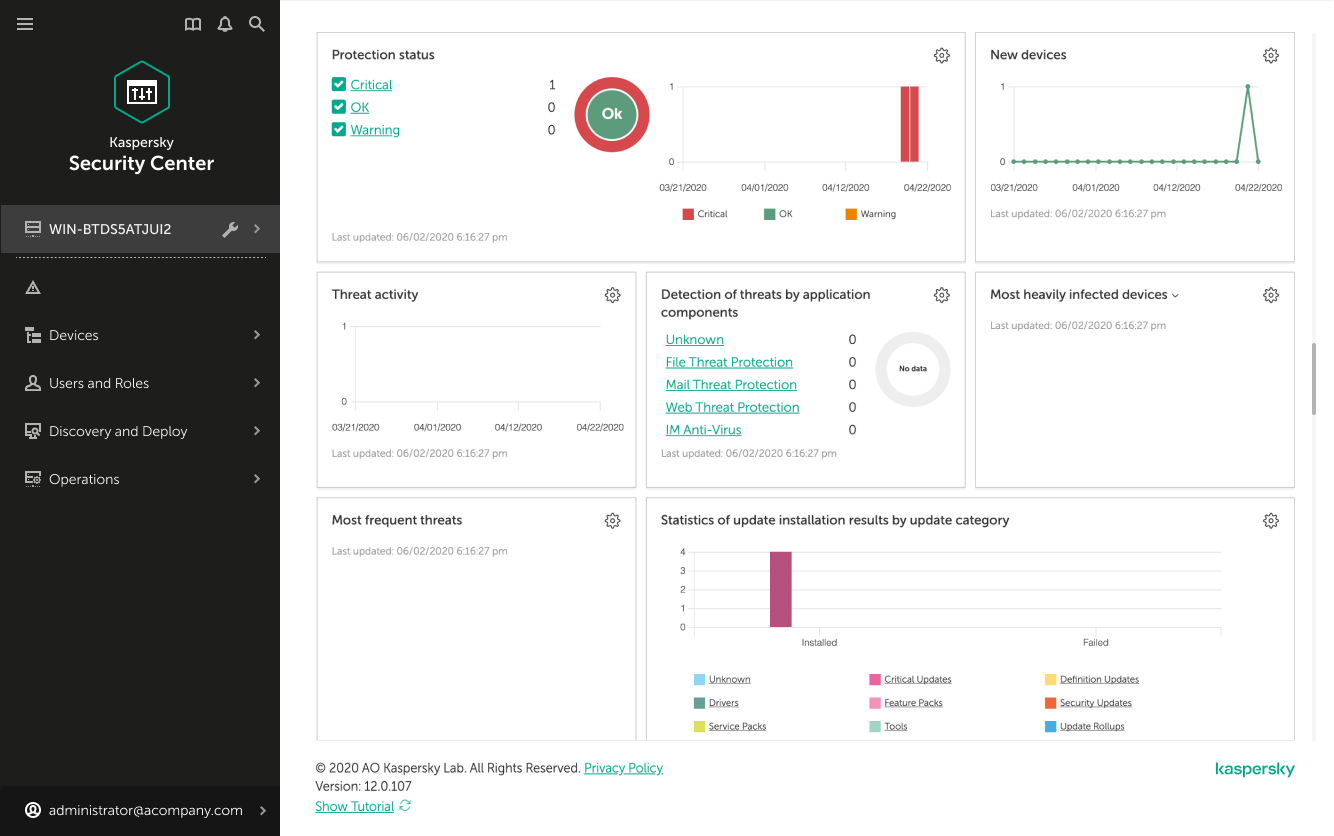
\includegraphics{images/KasperskySC.png}
         \caption{Kaspersky Security Center}
         \label{fig:KasperskySC}
      \end{figure}
   \end{itemize}
   \item \textbf{Discovery} - \textit{Obtener información y datos sobre el sistema}
   \begin{itemize}
      \item A través del componente infectado, el atacante puede \textbf{escanear} la red y obtener información sobre los dispositivos ciber y ciberfísicos conectados, lo que le permite establecer las vulnerabilidades actuales y planificar futuros ataques explotándolas.
      A menudo las comunicaciones entre dispositivos ciberfísicos y ciber carecen de \textbf{encriptación}, potencialmente exponiendo datos y credenciales sensibles.\\
      Si no hay suficiente segmentación de red, o si falta apropiada configuración de los Firewalls, este proceso puede ser aún más facilitado.
      \item \textit{\ul{Defensa}} - \textsc{KICS} for Networks detecta un escaneo de red no autorizado y envía una alerta a Kaspersky Security Center. Imagino que \textsc{KICS} también puede detectar cualquier movimiento lateral del atacante.
   \end{itemize}
   \item \textbf{Technlogical Attack} - \textit{Ataque a la infraestructura}
   \begin{itemize}
      \item Si no se bloquea el ataque en la fase anterior, el atacante puede enviar \textbf{comandos no autorizados} (\textit{command injection}) a los dispositivos ciberfísicos.\\
      El ejemplo que se hace en el video es de utilizar una vulnerabilidad ---conocida--- del firmware del componente de protección del transformador para enviar un comando inapropiado para updatear el firmware de modo que el dispositivo deje de cumplir su función de protección.

      \note{Vulnerabilidades típicas de sistemas CPS incluyen:\ns
      \begin{itemize}
      	\item Permissions, Privileges and Access Control
	      \item Improper Authentication
	      \item Insufficient Verification of Data Authenticity
      \end{itemize}
      Parece claro como estas pueden facilitar un ataque como el que se muestra en el video.}
      \item En este punto, el atacante puede causar daños físicos como cortocircuitos y similares
      \item \textit{\ul{Defensa}} - \textsc{KICS} for Networks detecta un comando no autorizado y envía una alerta a Kaspersky Security Center.\\
      Aunque no se detenga el ataque, podemos utilizar la información recopilada para mitigar futuros ataques.
   \end{itemize}
\end{enumerate}

% \framedt{
%    GOOSE spoofing
% }{
%    GOOSE spoofing es un ataque que consiste en enviar mensajes GOOSE (Generic Object Oriented Substation Event) falsos a los dispositivos de la subestación, lo que puede provocar fallos en el sistema.
% }

\subsection{Conclusiones sobre \textsc{KICS}}
El vídeo no discute en profundidad la defensa de \textsc{KICS}, pero me parece que el punto de fuerza de \textsc{KICS} sea que puede operar a diversos \textbf{niveles}, y que instancias de \textsc{KICS} pueden \textbf{comunicarse} entre sí para compartir información sobre ataques y vulnerabilidades.
Esto permite de hacer un análisis de lo que está ocurriendo más \textbf{completa} y \textbf{amplia}, que es el punto fundamental de la Ciberconciencia Situacional.

Sin embargo, el problema fundamental en sistemas ICS es que luego de detectar un ataque, hay que decidir como responder a él, porque \ul{no se puede hacer nada que pueda interrumpir o alterar el funcionamiento del sístema}, las prioridades son la continuidad del servicio, y la seguridad del personal y de la infraestructura.\\
Esto es un problema que no se discute en el video y cuya gestión puede depender mucho del sistema concreto en cuestión.